\documentclass[%
 preprint,            % For two-column layout
 superscriptaddress, % Affiliations with superscripts
 amsmath,amssymb,    % Math packages
 aps,                % APS style
 pra,                % Choose journal: prl, pra, prb, prc, prd, pre, prstab, prstper, rmp
 floatfix,           % Fixes for floating figures/tables
]{revtex4-2}

% ---------- Encoding ----------
\usepackage[T1]{fontenc}
\usepackage[utf8]{inputenc}

% ---------- Figures and graphics ----------
\usepackage{graphicx}   % Include figures
\usepackage{dcolumn}    % Align table columns on decimal point
\usepackage{bm}         % Bold math
\usepackage{xcolor}     % Colors

% ---------- References and links ----------
\usepackage[colorlinks=true, allcolors=blue]{hyperref}
\usepackage{cleveref}   % Smart cross-references

% ---------- Extra math ----------
\usepackage{mathtools}  % Extends amsmath
\usepackage{amsmath}
\usepackage{mathrsfs}

% ---------- Theorem-like environments (if needed) ----------
\usepackage{amsthm}
\newtheorem{theorem}{Theorem}
\newtheorem{lemma}{Lemma}
\newtheorem{definition}{Definition}

% ---------- Title info (example) ----------
\begin{document}

\title{Ecological Dominance and Hidden Neutrality in Global Diatom Communities}
\author{Emanuele Pigani}
\email{epigani@ictp.it}
\affiliation{Institute or University, Department, City, Country}
\author{Kobe Simoens}
\affiliation{Another Institute, City, Country}

\date{\today}

\begin{abstract}
    Astract
\end{abstract}

\maketitle

\begin{figure}
    \centering
    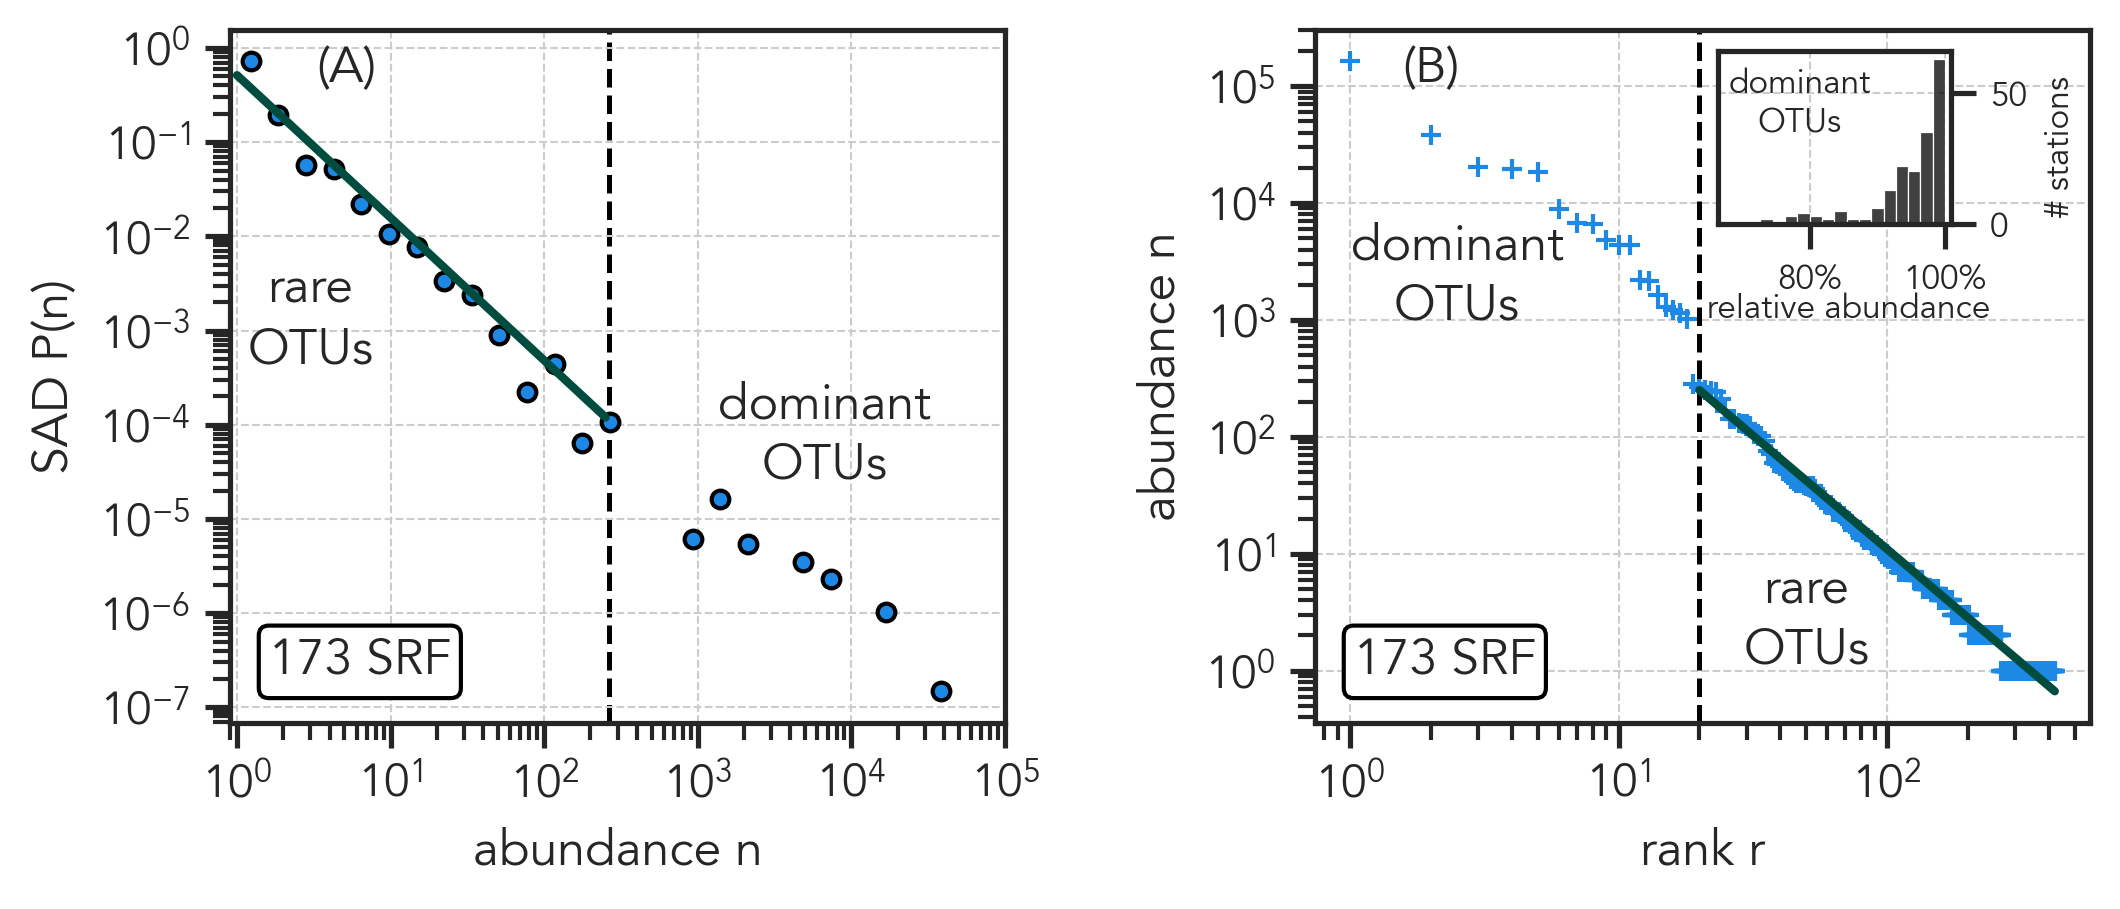
\includegraphics[width=0.95\linewidth]{fig/173_SRF_SAD_RAD.png}
    \caption{\textbf{Abundance and Rank-Abundance Distributions at Station \#173.}
        Panel (A): The SAD is divided into 20 dominant species (right), accounting for $99\%$ of the total abundance, and 246 non-dominant species (left). Non-dominant species follow a power-law distribution consistent with the neutral model, while dominant species show substantial deviations. 
        Panel (B): The rank-abundance distribution shows similar patterns, with dominant species (ranks $1$–$20$) deviating from neutral predictions, while non-dominant species align closely.}
    \label{fig:placeholder}
\end{figure}

\begin{figure}
    \centering
    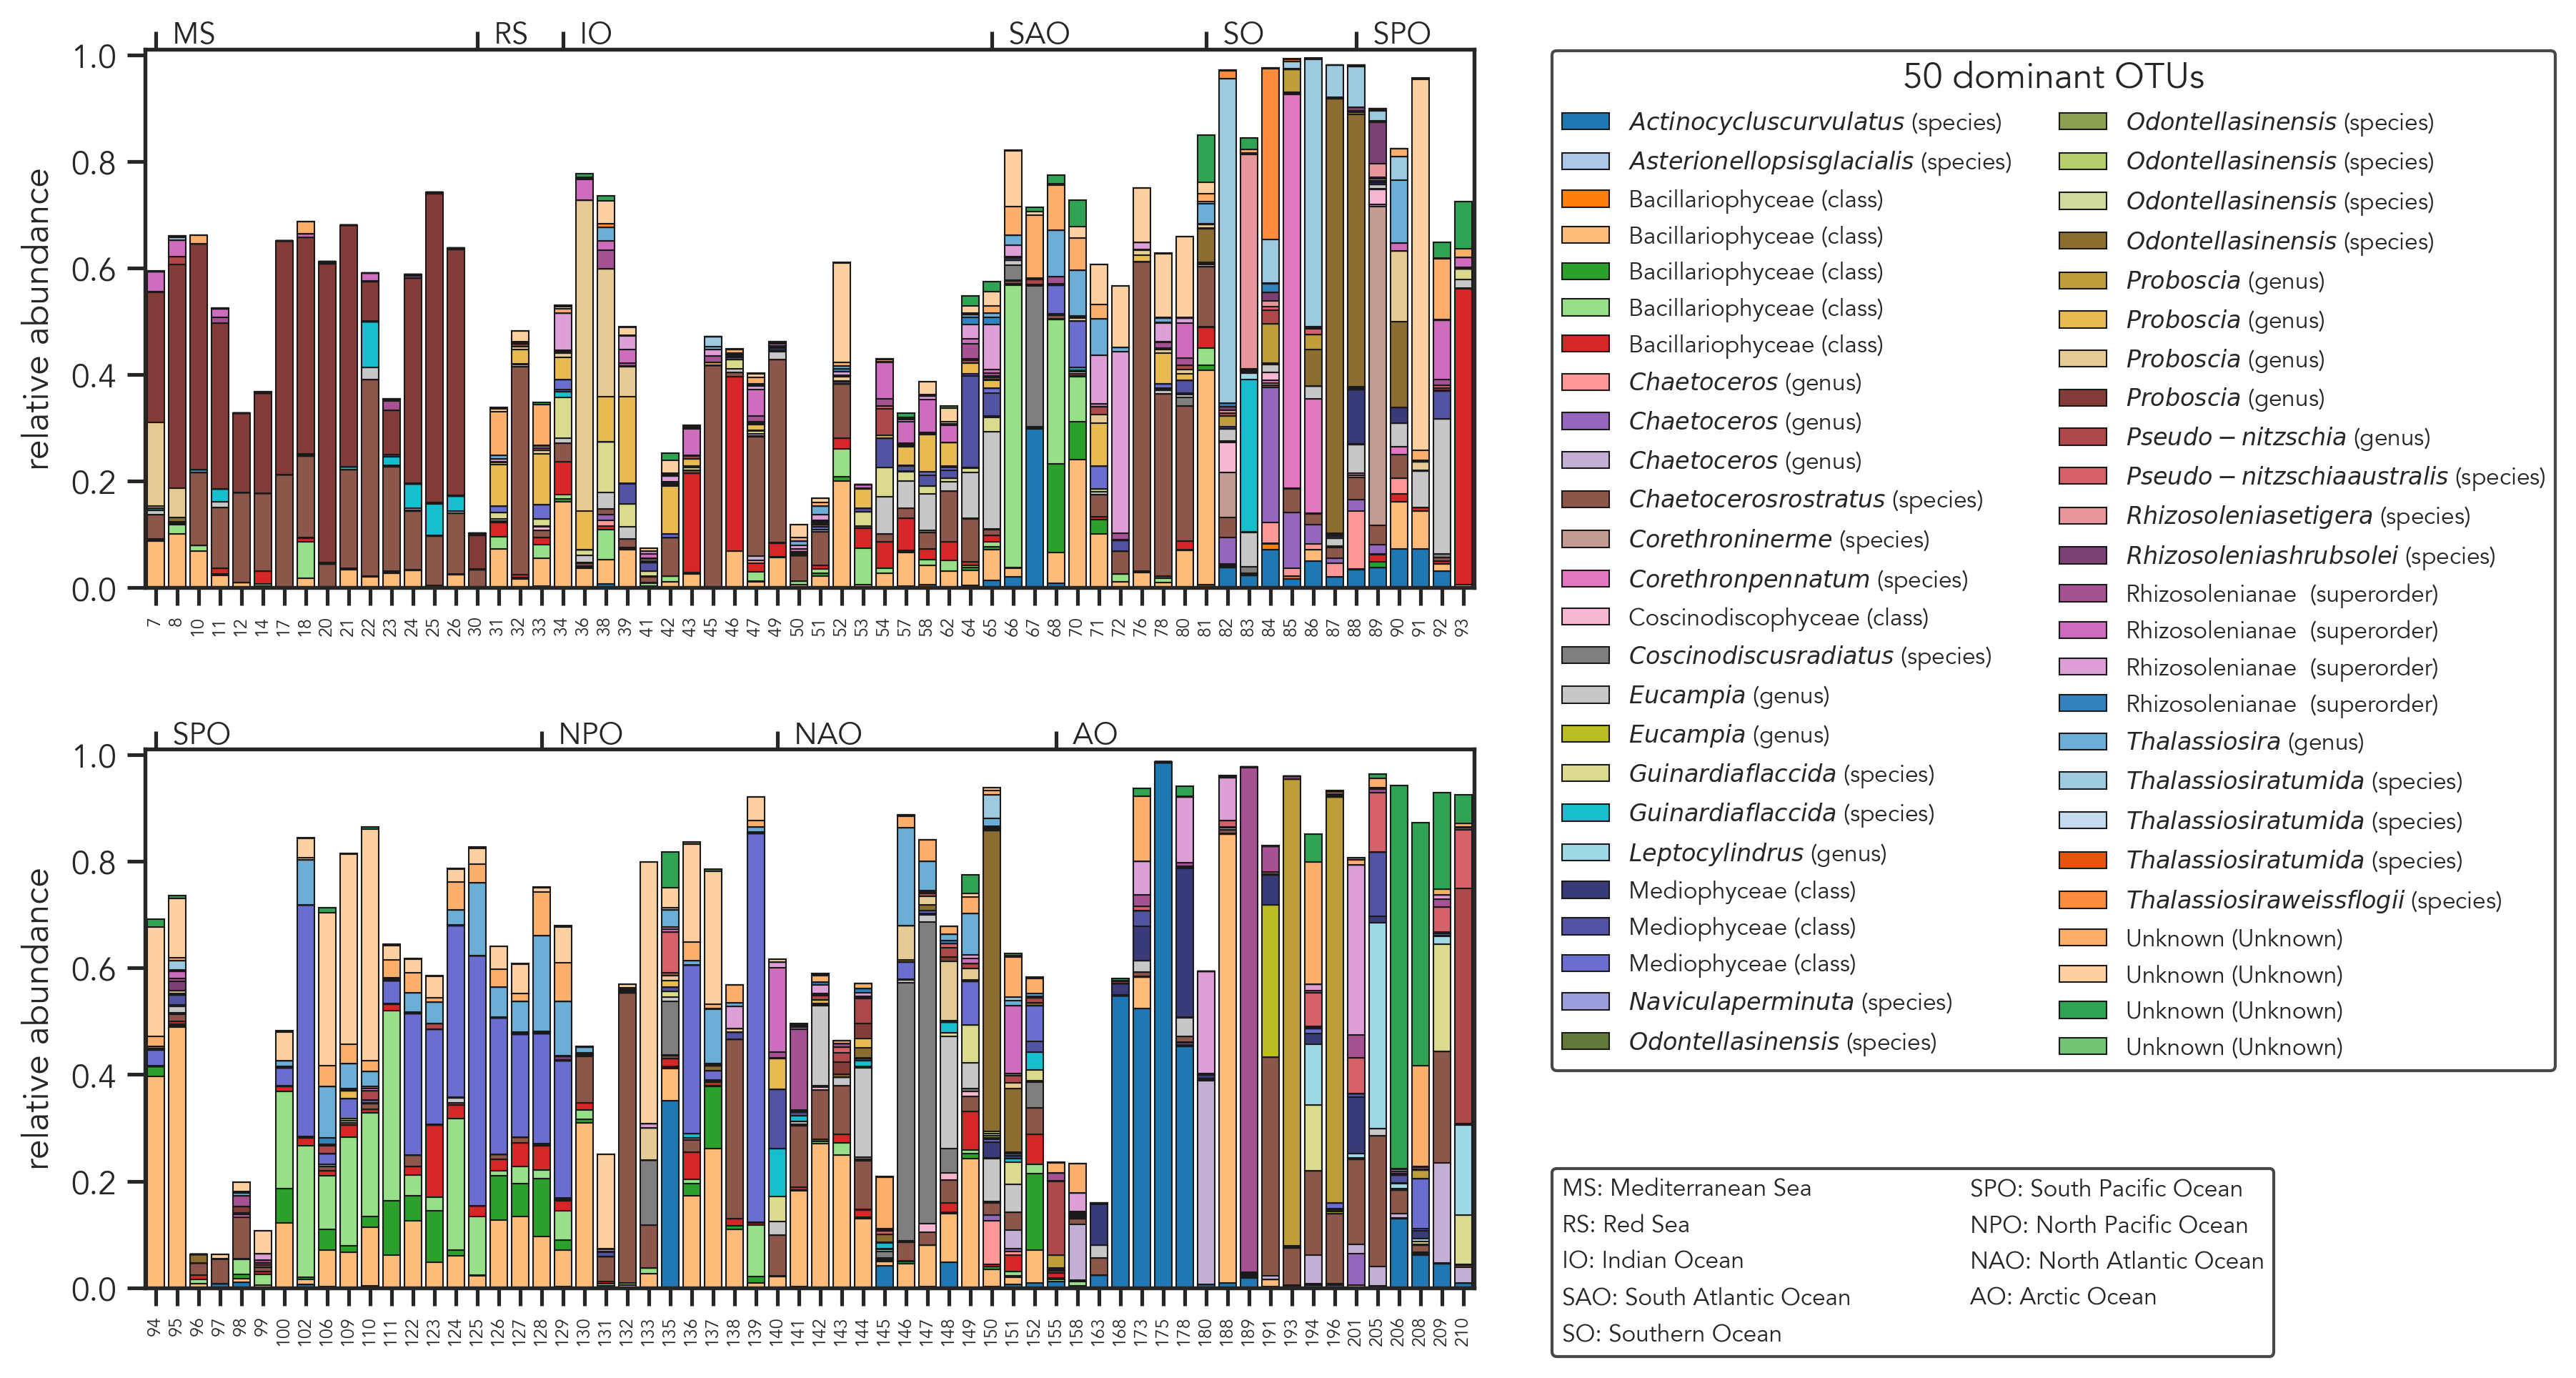
\includegraphics[width=0.95\linewidth]{fig/OTU_abundance_stacked_bar_chart.png}
    \caption{\textbf{Relative contributions of the 50 dominant OTU across stations.} Each bar represents one OTU, and each column is a station. OTU classifications are shown in the legend; some OTUs remain unclassified at the species level. Stations are grouped by oceanic basins for regional comparison.}
    \label{fig:placeholder}
\end{figure}

\begin{figure}
    \centering
    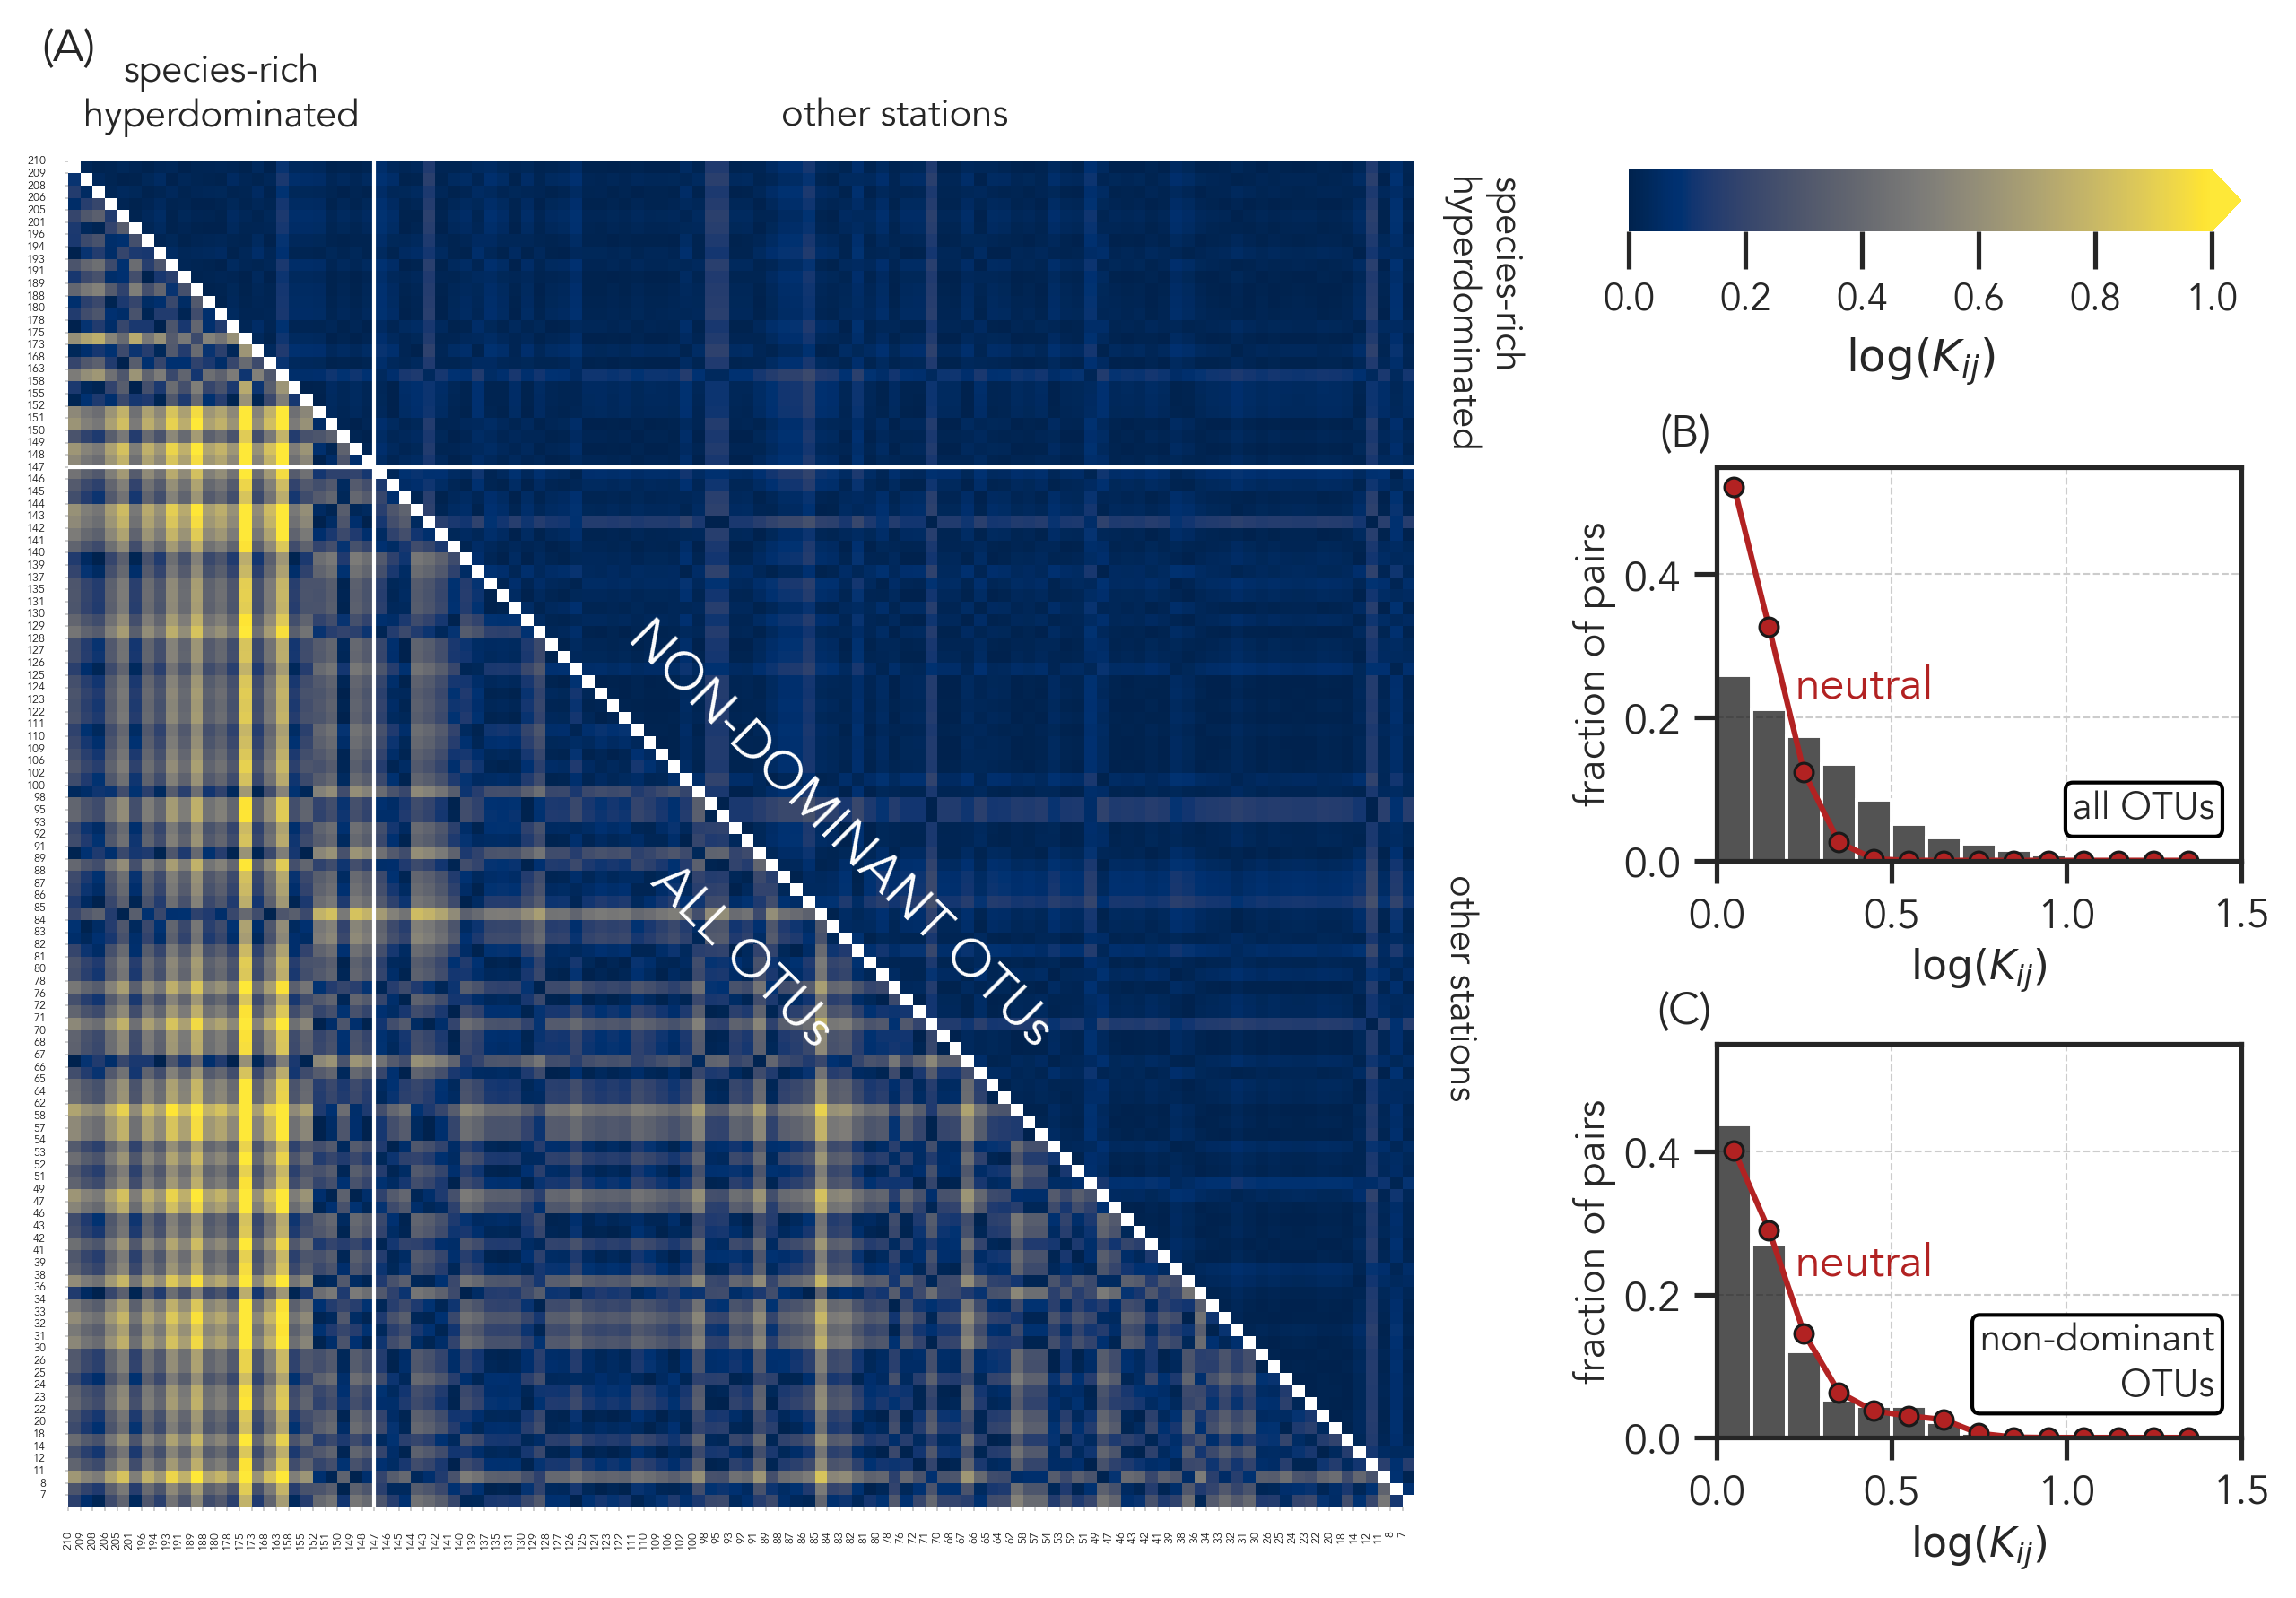
\includegraphics[width=0.95\linewidth]{fig/Hyperdominated_K_log_distance.png}
    \caption{\textbf{Relative contributions of the 50 dominant OTU across stations.} Each bar represents one OTU, and each column is a station. OTU classifications are shown in the legend; some OTUs remain unclassified at the species level. Stations are grouped by oceanic basins for regional comparison.}
    \label{fig:placeholder}
\end{figure}

\begin{figure}
    \centering
    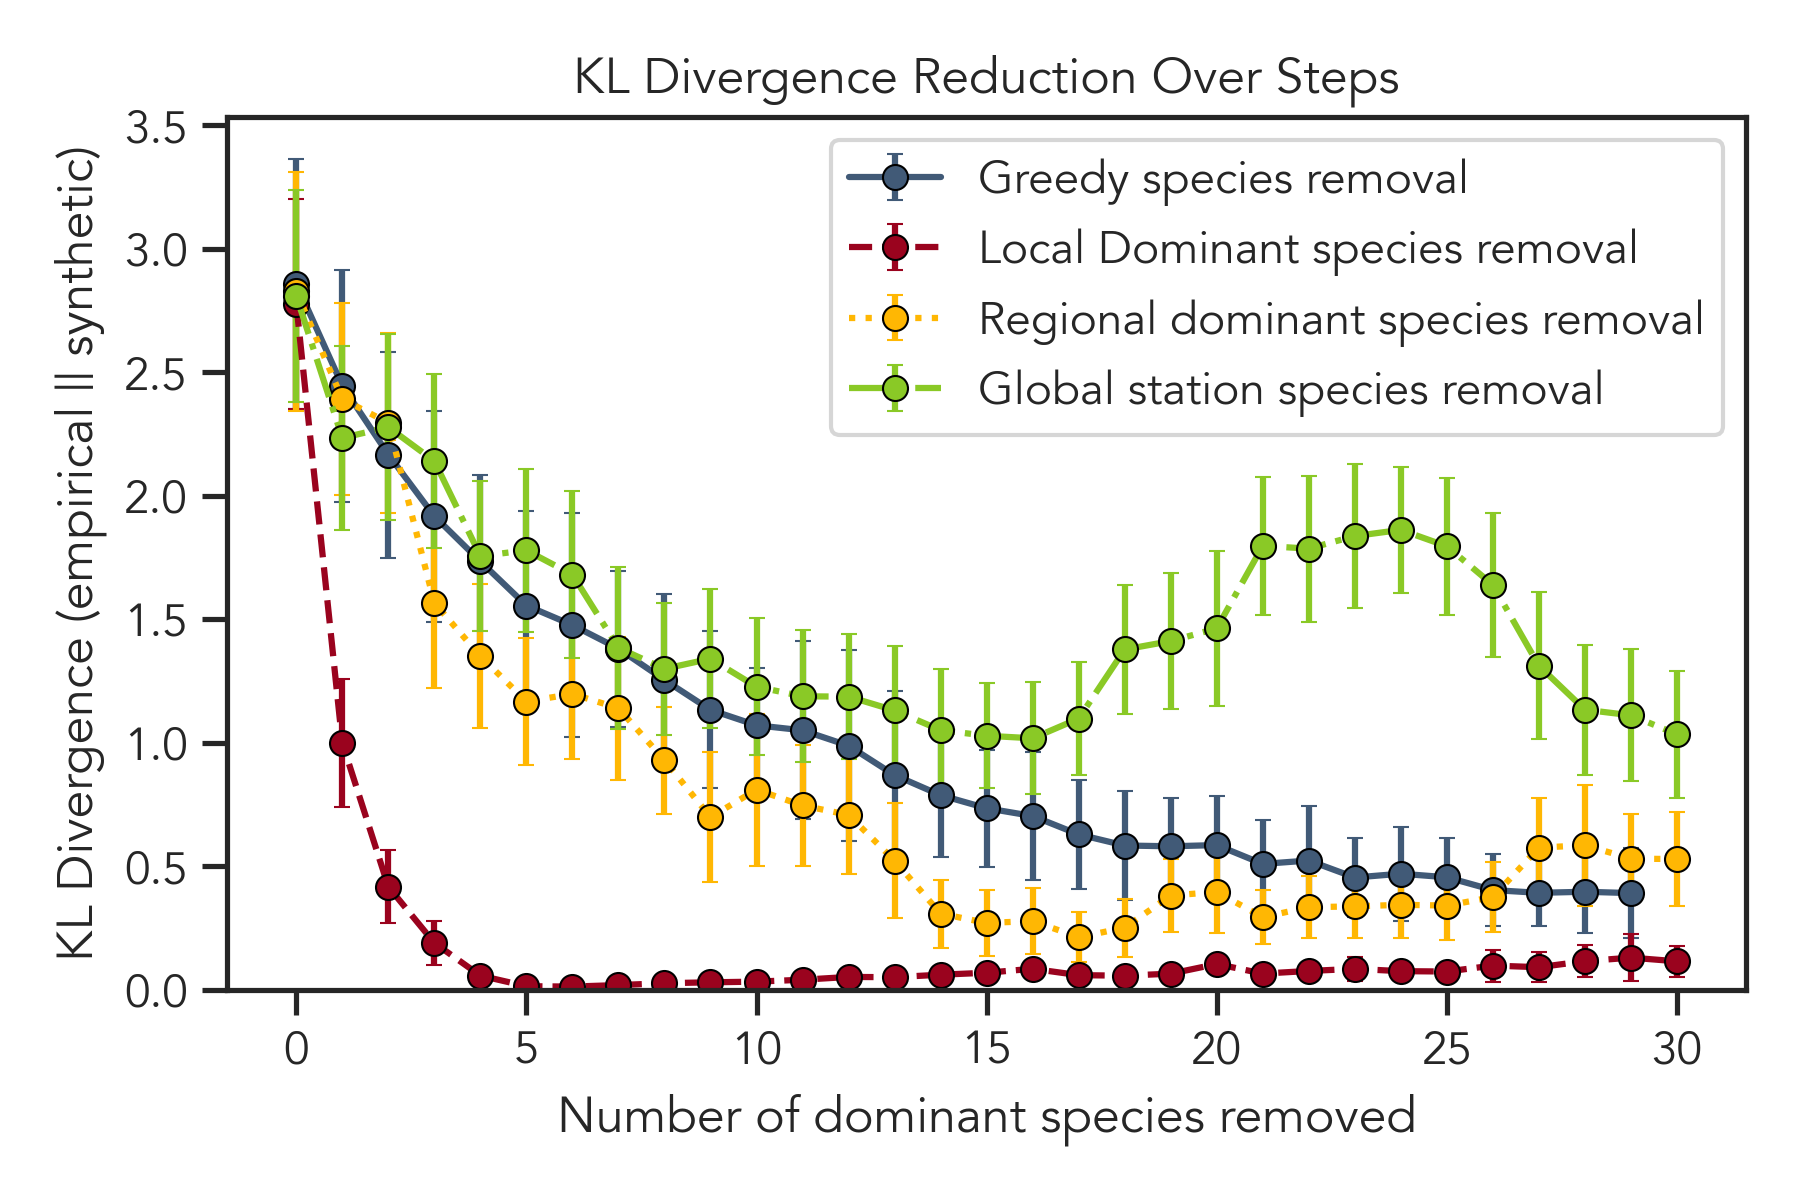
\includegraphics[width=0.75\linewidth]{fig/KL_divergence_reduction_comparison.png}
    \caption{\textbf{Reduction of Kullback–Leibler divergence between empirical and synthetic distributions as dominant species are progressively removed.} The KL divergence reaches its minimum after eliminating approximately the top five dominant species. Four removal strategies are compared: (blue) greedy removal, where species are iteratively removed across all stations to maximize the reduction in KL divergence; (red) local removal, where the $n$ most abundant species are removed independently at each station; (yellow) regional removal, where the $n$ most abundant species are removed at the scale of each ocean basin; and (green) global removal, where the $n$ most abundant species are removed based on their total abundance across all stations. The local removal strategy consistently yields the strongest and fastest reduction in KL divergence. This indicates that deviations from neutrality are driven primarily by locally dominant species, rather than by particular taxa, since the same species may follow neutral behavior in other stations. The KL divergence reaches its minimum after eliminating approximately the top five dominant species. Error bars indicate variability across different synthetic realizations.}
    \label{fig:placeholder}
\end{figure}

\appendix

\section{Birth-and-death Neutral Model}

We consider the birth-and-death Master Equation
\begin{equation}
    \partial_t P_{n}(t) = d_{n+1} P_{n+1}(t) + b_{n-1} P_{n-1}(t) - [d_n + b_n] P_{n}(t),
    \label{eq:app:BD-ME}
\end{equation}
where $P_n(t)$ represents the probability that the abundance of a focal species is $n$ at time $t$. Following~\cite{he2005deriving, sergiacomi2018ubiquitous, pigani2024deviation}, we assume that the birth and death rates are given by 
\begin{align}
        b_n &= b\, n + \chi, \label{eq:app:BD-model-b}\\
        d_n &= d\, n + \mu \left(1-\delta_{n,0}\right). \label{eq:app:BD-model-d}
\end{align}
The stationary solution can be derived analytically~\cite{he2005deriving}. For the sake of tractability within the broader framework developed below, we instead consider the diffusive limit, in which the Master Equation governing the system dynamics is approximated by the following Fokker–Planck equation:
\begin{equation}
    \partial_t P_n(t) = \partial_n \left[\left((b_1-d_1)n + b_0 - d_0)\right) P_n(t)(t)
    - \frac{1}{2} \partial_n \left[\left(\sigma_d n + \sigma_e) \right)P_n(t)\right]
    \right].
\end{equation}
The parameter $\sigma_d = d_1 + b_1$ quantifies demographic noise arising from birth-death processes, while $\sigma_e = d_0 + b_0$ captures environmental noise from external factors. 

The stationary solution to the Fokker-Planck equation reads:
\begin{equation}
    P_n= \mathcal{N} \left(1+\frac{n}{k}\right)^{-\lambda} e^{-\beta\, n}
    \label{eq:SAD-mG}
\end{equation}
where $\mathcal{N}$ is a normalization constant and the parameters are defined as:
\begin{equation}
    \begin{aligned}
        k&=\frac{\sigma_e}{\sigma_d }=\frac{b_0+d_0}{b_1+d_1},\\
        \lambda &= 1 + 4 \frac{d_0 b_1 - b_0 d_1}{(b_1+d_1)^2}, \\
        \beta &= 2 \frac{d_1-b_1}{d_1+b_1}.
    \end{aligned}
    \label{eq:params-mG}
\end{equation}
The distribution exhibits three distinct regimes: for $n \ll k$ it is nearly flat; in the intermediate range, $k < n < \beta^{-1}$, it follows a power law, which is subsequently bent by an exponential cut-off.

Considering taxonomic resolution, typical values of $d_0/d_1$ and $b_0/b_1$ range between $0$ and $1$ across planktonic groups~\cite{sergiacomi2018ubiquitous}, suggesting that variability in the dynamics is primarily demographic. Under these conditions, $k$ remains low, so that only the power-law regime and the exponential cut-off are detectable. In the critical regime often assumed in neutral models, the exponential cut-off disappears, leaving a pure power-law form of the species abundance distribution, which can be written as

\begin{equation}
P(n) = \frac{n^{-\lambda}}{\zeta(\lambda)} , \label{eq:SAD-PL}
\end{equation}

where $\zeta(\cdot)$ is the Riemann zeta function.

\section{Neutral Sampling Theory from a power-law SAD}

Following \cite{pigani2024deviation}, we consider a metacommunity inhabiting an oceanic volume $V$, composed of $S$ species whose abundances follow Equation~\eqref{eq:SAD-PL}. In a homogeneously mixed system, a local community can be regarded as a sample of volume $V_p < V$ drawn from the metacommunity.

If species are homogeneously distributed with density $\rho$, a condition typically met when ecosystem resources are saturated~\cite{hubbel2001book}, the sampling effectiveness $p$ corresponds to the fraction of individuals sampled ($N_p/N$). In this case, the total population in the sampled station is $N_p = \rho V_p$, while the total abundance in the metacommunity is $N = \rho V$, yielding $p = N_p/N$.

Consider now a species represented by $n$ individuals in the whole population. Under the assumption of random sampling, the probability that this species is represented by $k$ individuals in the sub-sample $p$ follows a binomial distribution:
\begin{equation}
\mathcal{P}_{binom}\left(k|n,p\right) = \binom{n}{k}p^k \left(1-p\right)^{n-k}.
\label{eq:binomialmat}
\end{equation}
Hence, the probability $\phi(k|p)$ that a species has an abundance $k\geq1$ at a sub-scale $p$ is the marginalization of the binomial over all the possible total abundances $n$ of the species at the global scale, i.e., $\phi(k|p) = \sum_{n\geq k} \mathcal{P}_{binom}\left(k|n,p\right) P_n$. The resulting local SAD is reported in \cite{pigani2024deviation}. Analogously, we can calculate the probability $\phi(k=0|p)$ that the species is not present at the local scale, with the only difference that now $n$ should be strictly larger than $0$. The probability for the focal species of not being present at the local scale reads
\begin{equation}
    \phi(0|p) =\frac{\text{Li}_{\lambda}(1-p)}{\zeta (\lambda)}
    \label{eq:phi0}
\end{equation}
where $\text{Li}$ is the polylogarithm function $\text{Li}_n(z)=\sum _{k=1}^{\infty } \frac{z^k}{k^n}$. If we assume $p\ll1$, i.e., the local sample represents a tiny fraction of the global metacommunity, we can expand \eqref{eq:phi0} and get a scaling relation for the richness (see \cite{pigani2024deviation}). Since $\lambda$ is typically close to $1.5$~\cite{sergiacomi2018ubiquitous}, we can explicitly write a scaling relation from the metacommunity properties as
\begin{equation}
    \langle S_p \rangle =      \underbrace{-\frac{\Gamma (-\lambda+1 )}{\zeta (\lambda)} \frac{S}{(N)^{\lambda-1}}}_{K} (N_p)^{\lambda-1},
    \label{eq:HeapsTaraMM}
\end{equation}
where $K$ is the \emph{metacommunity biodiversity index}, which is a function of the metacommunity properties. We can infer $K$ from the sampling data, provided that we know $\lambda$, as
\begin{equation}
    K = \frac{S_{loc}}{N_{loc}^{\lambda-1}},
    \label{eq:K-metacom}
\end{equation}
where $S_{loc}$ and $N_{loc}$ are the observed local richness and abundance, respectively. 

\section{Testing the hypothesis of a global neutral metacommunity}

Equation \eqref{eq:K-metacom} allows us to assess the existence of a global metacommunity and explore potential local metacommunities. If multiple metacommunities exist on intermediate spatial scales, we expect $K_i$ to remain consistent within clusters of stations belonging to the same metacommunity.

To examine the relationships between different metacommunities, we consider the ratio of their biodiversityindices. We define the \emph{biodiversity log-ratio distance} between metacommunities inferred from stations $i$ and $j$ as:

\begin{equation}
    \log K_{ij} = \lvert\log_{10}{K_i}-\log_{10}{K_j}\rvert
\end{equation}

If two stations belong to the same metacommunity, we expect $\log K_{ij} = 0$. The distribution of $\log K_{ij}$ values provides insight into the similarity of the stations and the potential existence of multiple metacommunities. 

\section{Estimating global richness}

On average, the neutral components of the communities represent a fraction $ N_{NT} / N_{TOT} = 1 / (1 + \alpha) $ of the total abundance, while they account for $ S_{NT} / S_{TOT} = 1 / (1 + \varepsilon) $ of the total richness. Here, $ N_{TOT} $ and $ S_{TOT} $ denote the total number of individuals and species (or OTUs), respectively, while $ N_{NT} $ and $ S_{NT} $ refer to the corresponding quantities restricted to the neutral component, as defined by our model-based filtering procedure. The parameters $ \alpha > 0 $ and $ \varepsilon > 0 $ quantify the relative contributions of non-neutral individuals and species, respectively. ADD ESTIMATES FROM DATA.
Combining this with the theoretical scaling derived in Equation~\eqref{eq:HeapsTaraMM} for the neutral component,
we obtain a corresponding prediction for the total richness:
\begin{equation}
    S_{TOT} = K \frac{1+\varepsilon}{(1+\alpha)^{\lambda-1}} \frac{-\zeta(\lambda)}{\Gamma(1-\lambda)}  (N_{TOT})^{\lambda -1}.
    \label{eq:global-heaps}
\end{equation}

TODO 

To estimate the total number of diatom cells in the global ocean, we combined published estimates of total diatom biomass with an average carbon content per cell. Specifically, we used the following relationship:
\begin{equation}
    N_{\mathrm{TOT}} = \frac{B_{\mathrm{TOT}}}{\langle C_{\mathrm{cell}} \rangle}
\end{equation}

where $ N_{\mathrm{TOT}} $ is the total number of diatom cells, $ B_{\mathrm{TOT}} $ is the total diatom biomass expressed in units of carbon (e.g., grams of carbon), and $ \langle C_{\mathrm{cell}} \rangle $ is the mean carbon content per diatom cell. Estimates of $ B_{\mathrm{TOT}} \approx 5 \times 10^{14}\, \textrm{g C}$ were taken from large-scale oceanographic surveys and global models~\cite{leblanc2012global},
while $ \langle C_{\mathrm{cell}} \rangle  \approx 10^{-8} \, \textrm{g C cell}^{-1} $ was derived from \cite{linacre2021cell}. Together, this gives an estimate for $N_{\mathrm{TOT}} \approx 10^{23} \textrm{cell}$.

\section{Reconciling the inverted paradox}





% ---------- Bibliography ----------
\bibliographystyle{apsrev4-2}
\bibliography{biblio}

\end{document}